\chapter{Contexte}
\label{chpt:contexte}
    
    \section*{Table des Matières}
    \localtableofcontents
    
    \section{Garantir la sécurité d'un programme ou d'un système}
    
        La sûreté et la sécurité des programmes et des systèmes sont des enjeux majeurs de nos jours. 
        
        La \textit{sûreté} se réfère à l'ensemble des risques dont la cause est accidentelle. La \textit{sécurité} concerne quant à elle les actes de malveillance.
        Si on prend pour analogie un aéroport, la panne d'un avion correspond à un risque de l'ordre de la sûreté tandis qu'un attentat relève de la sécurité.
        Une \textit{attaque} correspond à une tentative d'un adversaire (appelé \textit{attaquant}) d'obtenir un avantage sur un système. 
        Cet avantage peut se traduire par une élévation de privilèges \cite{Timmers/FDTC16} ou l'accès à des données sensibles \cite{Biham/AICC97} par exemple, mais dans un cadre général il peut s'agir de tout comportement qui n'a pas été prévu pour le système. 
        Par \textit{système} nous entendrons de manière générique un appareil informatique, un programme, un réseau de sous-systèmes et plus généralement, toute entité traitant de l'information répondant à des besoins de sûreté et susceptible d'être attaquée.
        
        Des ordinateurs aux téléphones modernes, en passant par les appareils connectés ou encore les cartes à puces, le nombre de systèmes et de technologies disponibles continue de croître \cite{HardwareEmbeddedSystems}. La surface d'attaque globale ne cesse donc de grandir, et la diversité des attaques qui doivent être prises en compte lors de la mise en place d'un système rend le processus de développement plus complexe. 
        
        Pour parer à ces menaces, des protections sont mises en oeuvre de manière à détecter ou bloquer les attaques. Ces protections peuvent prendre la forme de transformations du programme source, par exemple en modifiant l'algorithme \cite{Aumuller/CHES02} ou en rajoutant du code visant à détecter et/ou empêcher les attaques  \cite{Reis/ISCCO05, lalande}. Les protections peuvent aussi être appliquées au niveau de la plateforme, comme par exemple la randomisation de l'espace mémoire par le système d'exploitation de manière à rendre l'exploitation des attaques plus difficiles \cite{shacham2004effectiveness}. Ou encore, au niveau matériel, en ajoutant des protections physiques dans le composant de manière à limiter la lecture des données stockées \cite{Boneh/EUROCRYPT97}.
        
        De nouvelles attaques sont découvertes et mènent à la recherche de nouvelles protections qui sont par la suite attaquées à leur tour. Ainsi, les attaquants se diversifient et un système doit faire face à des menaces variées. 
        
        \begin{probl}
        \label{prob:help-dev}
            Comment faciliter le processus de développement d'un logiciel afin d'aider le développeur dans le choix et la mise en place des protections ?
        \end{probl}
        
        Plus encore, une nouvelle attaque peut être découverte après l'analyse de la sécurité d'un programme et ainsi mettre en lumière de nouvelles vulnérabilités. Les processus d'évaluation et de protection d'un système doivent donc être réexaminés à intervalles réguliers de manière à prendre en compte les nouvelles menaces. 
        
        Bien entendu, le niveau de sécurité dépend grandement du contexte d'utilisation d'un système. La confidentialité des communications d'un satellite militaire doit répondre à un niveau de sécurité plus élevé que celle d'une boite au lettre d'un particulier par exemple. A l'inverse, une serrure pour une résidence est une protection contre les tentatives d'intrusion dont la nécessité est discutable pour un satellite. Il est nécessaire d'évaluer le risque d'une attaque en fonction du niveau de sécurité qu'on souhaite atteindre et en fonction du système à protéger. La balance bénéfice/coût de l'attaquant est à prendre en compte par le défenseur pour évaluer les menaces du système.
        
        Pour permettre de certifier la sûreté et la sécurité d'un système, des méthodologies ont été développées. La certification \gls{cc} \cite{CommonCriteria17} est un processus de certification standardisé par la norme \gls{iso} 15408 permettant à des organismes spécialisés de garantir un certain niveau de sécurité sur un système. Les \gls{cc} proposent un ensemble de procédures permettant d'obtenir un niveau d'assurance sur la sécurité du système en question. Ainsi, il est possible de viser un type de certification en fonction du niveau de sécurité voulu. La figure \ref{tbl:common-criterias-levels} présente les différents niveaux d'assurance des \gls{cc}, chacun définissant un seuil de mise en place de moyens humains, d'expertise et de technologie par le fournisseur du produit et l'organisme de certification et des critères en fonction des problèmes découverts pour l'obtention ou non du certificat. 
        
        \begin{table}
        {\small
            \begin{center}
\begin{tabular}{cc}
\hline
EAL  & Description                                     \\ \hline
EAL1 & Testé fonctionnellement                         \\
EAL2 & Testé structurellement                          \\
EAL3 & Méthodiquement testé et vérifié                 \\
EAL4 & Méthodiquement conçu, testé et revu             \\
EAL5 & Semi-formellement conçu et testé                \\
EAL6 & Conception semi-formellement vérifiée et testée \\
EAL7 & Conception formellement vérifiée et testée      \\ \hline
\end{tabular}
            \end{center}
            }
                \caption{Les différents niveaux de certification des Critères Communs \cite{Dureuil/Phd16}}
                \label{tbl:common-criterias-levels}
\end{table}

        De la même manière, les audits de sécurité sont effectués pour les systèmes d'information et mettent en place des scénarios d'attaque variés de manière à s'assurer de la sécurité du système. Des tests d'intrusion (les \textit{pentests}) sont mis en oeuvre afin de simuler différents types d'attaquant et de vérifier la réaction du système.  
        Différents modèles d'attaquant sont considérés, en allant du test en boite noire où le système est inconnu de l'attaquant et qui se place à l'extérieur de celui-ci, au test en boite blanche où l'attaquant est modélisé comme connaissant les détails internes du système ou comme ayant un accès privilégié dans le système. 
        
        \begin{probl}
        \label{prob:help-auditor}
            Comment faciliter le processus d'évaluation par l'expert d'un programme et de ses protections à l'aide de méthodologies et d'outils ?
        \end{probl}
        
        La sécurité a un coût, à la fois en termes de moyens humains et d'expertise mais également parce que les protections peuvent complexifier le système, ou altérer les performances (rapidité d'exécution inférieure, taille du code plus grande...). De plus, d'autres problématiques industrielles comme des délais de production ou des limitation matérielles viennent se combiner à celle de la sécurité. 
        Par exemple, les processeurs modernes utilisent une optimisation appelée l'exécution spéculative qui vise à exécuter une branche d'un programme avant que la condition de branchement soit évaluée. Si la mauvaise branche a été choisie, la pipeline est déroulée pour revenir à son état précédent pour exécuter la bonne branche. Cette technique permet de fournir une performance accrue pour le processeur. Néanmoins, l'attaque Spectre, découverte en 2019 \cite{Kocher/SP2019}, a démontré qu'il était possible d'exploiter les effets de bord de cette optimisation de manière à retrouver des informations secrètes qui ne sont normalement pas accessibles. Un compromis est souvent nécessaire entre les différentes problématiques (sûreté, sécurité, performance, accessibilité etc.) liées au développement d'un système.
        
        Chaque couche ou noeud d'un système pouvant être menacé, une attaque peut être composée de plusieurs attaques visant des parties différentes du système. Par exemple, l'attaque \textit{Rowhammer} \cite{Kim/ACM14, Park/IIRW14}, permet à un attaquant de tirer profit d'effets de bord dans le fonctionnement des cellules mémoires \gls{dram} pour augmenter le niveau de privilèges sur une machine sans nécessité d'accès physique. 
        Ce fut aussi le cas lors du challenge \textit{Wookey} \cite{SSTIC20} où un chemin d'attaque hybride a été détecté dans lequel la protection contre le dépassement de tampon implémentée dans l'interface de carte à puce (\gls{iso} 7816) est contournée par une attaque physique. La combinaison des deux attaques permet d'obtenir une élévation de privilège. 
        
        \begin{probl}
        \label{prob:high-order-analysis}
            Comment évaluer un programme et ses protections dans un contexte d'attaques multiples ?
        \end{probl}
        
        Cette thèse s'inscrit dans ce contexte et vise à proposer des solutions pour la protection et l'évaluation d'un programme et de ses protections. Ce chapitre présente des problématiques générales liées à l'analyse de programmes et de protections ainsi que les contributions apportées dans cette thèse. 

        \subsection*{L'exemple verify\_pin}
            
            Le programme présenté dans le listing \ref{lst:verifyPIN-BU} est une version naïve d'un processus de vérification de code \gls{pin} en langage C. Ce programme servira d'exemple pour présenter les enjeux et les problématiques de la protection et l'analyse de programmes. 
            
\lstset{caption={Programme verify\_pin \og naif \fg{} },label=lst:verifyPIN-BU}
\begin{lstlisting}
// PIN secret.
static uint8_t card_pin[5] = {'0', '1', '2', '3', '\0'}; 
static int try_counter = 3;

bool compare(uint8_t* a1, uint8_t* a2)
{
    int i = 0;
    while(*a1 != '\0') {
        if(*a1 != *a2)
            return false;

        ++a1; ++a2;
    }

    return true;
}

bool verify_pin(uint8_t* user_pin) { 
    if(try_counter > 0) {    
        if(compare(card_pin, user_pin)) {
            try_counter = 3;
            return true;
        } else {
            try_counter--;
            return false;
        }
    }

    return false;
}
\end{lstlisting}

        La figure \ref{fig:verifyPIN-spec} est un schéma d'utilisation fonctionnel de ce programme. L'authentification nécessite que le compteur d'essais soit strictement positif et que le \gls{pin} d'entrée soit identique à celui de la carte.
        Le programme \texttt{verify\_pin} est décomposé en deux: la fonction \texttt{verify\_pin} prend en argument le \gls{pin} utilisateur et appelle la fonction \texttt{compare} qui se charge de comparer les deux chaînes correspondant aux \gls{pin}s.        
        
        \begin{figure}[!ht]\centering
            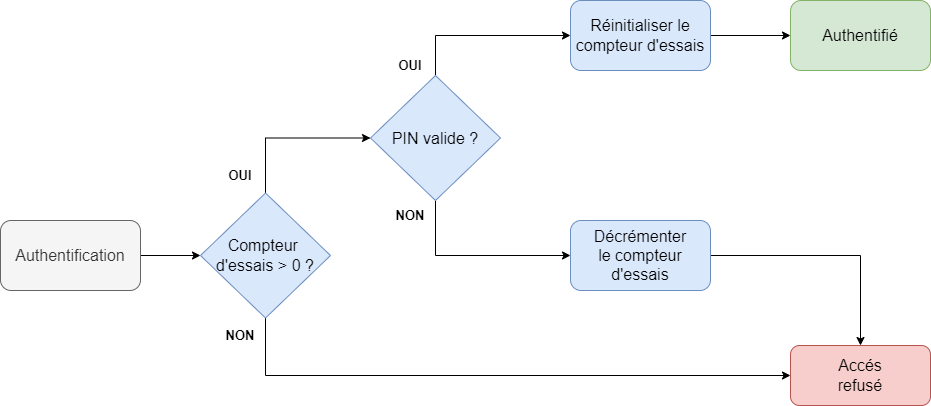
\includegraphics[scale=0.4]{ch1-context/img/verifyPINSpec.png}
            \caption{Schéma fonctionnel du programme \textit{verify\_pin}}  \label{fig:verifyPIN-spec}
        \end{figure}
        
        Dans la fonction principale, un compteur d'essai est vérifié de manière à limiter le nombre d'erreurs d'entrées successives autorisées. Le compteur est décrémenté en cas d'échec et remis à la valeur 3 lorsque l'authentification est un succès. Le \gls{pin} secret \texttt{card\_pin} est modélisé par un tableau statique pour cet exemple (ce qui n'est pas le cas dans la réalité).        
        
        La fonction \texttt{compare} effectue une comparaison de deux chaînes en bouclant sur chaque caractère jusqu'à atteindre un caractère terminant par le caractère nul `\textbackslash0'. Si deux caractères sont différents, la boucle se termine prématurément en retournant \textit{faux}. Cela correspond à ce qui est fait par des fonctions C standards telles que \texttt{strcmp}.
        Les deux fonctions retournent des valeurs booléennes \textit{vrai} et \textit{faux} respectivement représentées par les entiers $1$ et $0$.
        
        Ce programme illustre une problématique d'authentification qui est présente dans un grand nombre d'objets sécurisés, par exemple les cartes \gls{sim} des téléphones ou les cartes à puces.     
        
    \section{Modèles d'attaquant et objectif d'attaque}
    \label{sec:model-attack}
    
        Lorsqu'on s'intéresse à la sécurité d'un programme, il est nécessaire de définir l'adversaire contre lequel on souhaite se protéger, ce qui se traduit par le \textit{modèle d'attaquant}.
        
        On aimerait dans l'idéal pouvoir rester le plus général possible, mais en pratique les outils et méthodes d'analyse restreignent le contexte dans lequel le programme est étudié. Cela est fait d'une part, pour maintenir des temps de calcul réalistes et d'autre part, parce qu'il n'y a pas de limite théorique à la puissance d'un attaquant, qui va dépendre du contexte et des moyens mis en oeuvre. Si un programme est sécurisé face à un modèle d'attaquant précis, rien n'empêche qu'un autre type d'attaque soit découvert par la suite et remette en question la sécurité du programme. 
        
        \begin{probl}
        \label{prob:attack-model}
            Comment définir et modéliser un attaquant dans le contexte d'une analyse de sécurité ?
        \end{probl}
        
        Le \textit{modèle d'attaquant} peut être vu comme un ensemble contenant : l'objectif d'attaque et le pouvoir de l'attaquant, comme présenté dans la figure \ref{fig:attacker-model}.
        
        \begin{figure}[!ht]\centering
            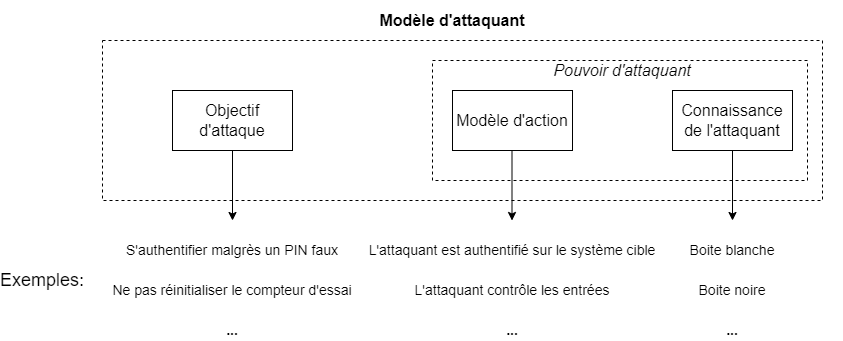
\includegraphics[width=\textwidth]{ch1-context/img/attack-model.png}
            \caption{Modèle d'attaquant}  \label{fig:attacker-model}
        \end{figure}
        
        On appelle \textit{objectif d'attaque} la propriété de sécurité visée par un adversaire. Pour l'exemple \textit{verify\_pin}, un objectif d'attaque naturel consiste à s'authentifier sans connaître le code de la carte. Un second objectif peut être de ne pas décrémenter le compteur d'essais lors d'un échec d'authentification. 
        
        On appelle \textit{modèle d'action}, l'ensemble des actions qu'un attaquant est capable d'effectuer sur le système cible. La \textit{surface d'attaque} correspond à l'ensemble des points du système sur lesquels l'attaquant effectue ses actions et est donc directement liée au modèle d'action considéré.
        
        Une \textit{vulnérabilité} est une faiblesse, dans une implémentation ou un système, pouvant être exploitée par un adversaire. Une vulnérabilité peut être un système mal configuré, non mis à jour, une erreur dans un logiciel, l'usage d'algorithme cryptographique non sûr ou même d'ordre organisationnel comme la présence d'un adversaire au sein du personnel de l'entreprise par exemple. Une vulnérabilité est intrinsèquement liée à un modèle d'attaquant, par exemple un programme peut être vulnérable aux dépassements de tampon ou à un défaut d'alimentation.
        
        On parle d'\textit{exploitation} pour désigner un programme ou une méthode permettant d'exploiter une vulnérabilité dans un système (en obtenant une élévation de privilège par exemple). La présence d'une vulnérabilité n'implique pas forcément qu'une exploitation soit possible dans l'immédiat. Par exemple, l'attaque \textit{Rowhammer} présentée précédemment a été d'abord théorisée \cite{Kim/ACM14} puis exploitée plus tard ~\cite{Seaborn/BH15,Gruss/DIMVA16}. Une vulnérabilité peut potentiellement être exploitée bien après sa découverte. Dans l'exemple \textit{verify\_pin}, une vulnérabilité sur la ré-initialisation du compteur de boucle en cas d'échec pourrait être exploitée pour obtenir un accès à la carte à l'aide d'une attaque par force brute.
        
        Enfin, le modèle d'attaquant inclus aussi la connaissance qu'un adversaire a sur sa cible, la \textit{connaissance de l'attaquant}. C'est ce que représente la diversité des tests en certification par exemple avec des attaquants agissant sur un système en boite noire ou en ayant un accès et une connaissance plus ou moins étendue sur le système. La \gls{jil} \cite{JIL} fait la distinction entre différents niveaux d'expertise reflétant la capacité d'un attaquant à utiliser des outils d'audit ou à créer de nouvelles attaques. Cette modélisation de la connaissance de l'adversaire sur le système permet aussi d'évaluer le risque que présente une vulnérabilité sur le système lors des processus d'audit. Un attaquant ayant un accès et des connaissances privilégiés sur le système est plus dangereux mais moins probable.
        
        En allant d'un attaquant ne contrôlant que les entrées du programme à un adversaire infiltré en tant d'administrateur sur la machine cible, le modèle d'attaquant peut radicalement varier en fonction du cadre d'usage du programme et des techniques d'attaques connues. Les exploitations peuvent mettre en oeuvre plusieurs types d'attaques, comme dans l'exemple \textit{Wookey} évoqué précédemment, et demande donc de prendre en compte des objectifs d'attaque variés.
        
        Dans le cadre de l'analyse logicielle, les outils et les techniques d'analyses doivent faire face à la diversité des modèles d'attaquants, bien que actuellement ils soient souvent spécifiques à des classes d'attaques particulières.
        
        \begin{probl}
            \label{prob:evolving-models}
            Comment faciliter l'analyse et la protection de programme pour des modèles d'attaquants qui évoluent et se complexifient ? 
        \end{probl}
        
    \section{Analyse de programmes}
    \label{sec:analysis}
        
        \begin{sloppypar}
        Le problème de l'arrêt énoncé par Alan Turing \cite{Turing/37} a montré qu'il n'existe pas de méthode d'analyse automatique permettant de savoir si un programme termine ou non. Lorsqu'on s'intéresse à la vérification de propriétés non triviales sur un programme, on se confronte au problème de l'indécidabilité \cite{Bradley/VMCAI06}. Toutefois, il existe des méthodes pour étudier le comportement d'un programme malgré cette limitation.
        \end{sloppypar}
        
        La fonction \texttt{foo} présentée dans le listing \ref{lst:foo-program} prend en entrée les variables $a$, $b$ et $c$ et calcule $a*b*c$. Même dans un cas simple comme celui-ci, il n'est pas trivial de s'assurer que la fonction se comporte toujours correctement.

\begin{lstlisting}[caption={Fonction foo}, label=lst:foo-program]
int foo(int a, int b, int c) {
    int total = 0;
    for(int i = 0; i < c; ++i)
        total += a * b;
    return total;
}
\end{lstlisting}        

        La fonction \textit{foo} possède un nombre fini d'\textit{exécutions} différentes possibles. Les entrées sont constituées seulement des trois variables  $a$, $b$ et $c$, mais il reste difficile de tester par force brute toutes les combinaisons d'entrées ($2^{96}$ possibilités dans le cas d'entiers codés sur 32 bits).
        Plus encore, certains programmes peuvent potentiellement avoir un nombre d'exécutions infinies. Le système peut attendre des entrées utilisateurs ou un évènement réseau sans limite finie, ce qui rend impossible l'exploration exhaustive des exécutions dans le cas de boucles ou de cycles infinis.
        
        Même si on pouvait effectuer une analyse exhaustive des exécutions, la question de la modélisation du système est aussi une problématique majeure. En effet, si on veut par exemple s'intéresser aux effets d'un dépassement de capacité du type entier dans la fonction \texttt{foo}, il faut prendre en compte l'encodage utilisé et les spécificités des architectures cibles. 
        Pour pallier ce problème, il est possible d'effectuer ces tests sur une véritable machine ce qui apporte des garanties concernant la précision de l'analyse mais nécessite la mise en place d'un banc de test physique et rend l'analyse spécifique au système de test choisi \cite{Faurax/Phd09}.
        
        De nombreuses techniques d'analyses ont été développées pour la vérification de programmes, que ce soit dans le domaine de la sécurité ou de la sûreté. Les méthodes d'analyses peuvent être classées en quatre catégories, présentées dans la figure \ref{fig:analysis-methods}, en fonction de leur approximation de l'ensemble des exécutions du programme étudié.
    
        \begin{figure}[!ht]
            \centering
            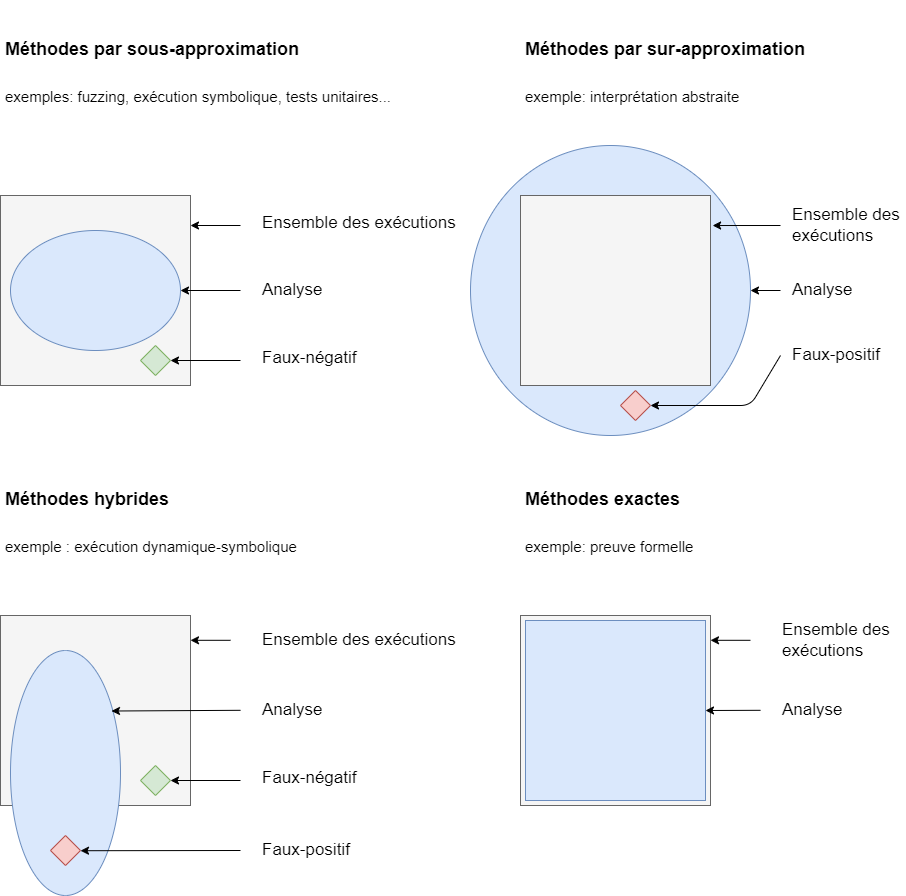
\includegraphics[scale=0.56]{ch1-context/img/analysis.drawio.fr.png}
            \caption{Méthodes d'analyses statiques} \label{fig:analysis-methods}           
        \end{figure}           
        
        Les \textit{méthodes par sous-approximations} étudient un sous-ensemble des exécutions possibles d'un programme. L'exemple naturel est le test. Les tests unitaires sont très utilisés en développement logiciel et consistent à tester indépendamment des fonctions et des modules d'un programme en se concentrant souvent sur les cas qui sont à priori susceptibles d'entraîner des erreurs (telles que les bornes du type des entrées ou des valeurs interdites par la spécification par exemple). 
        Le fuzzing \cite{Manes/TSE19} est une autre méthode de génération de test où les entrées sont choisies aléatoirement (ou semi-aléatoirement à l'aide d'heuristiques).
        L'exécution symbolique \cite{King/ACM76} (qui sera détaillé dans la section \ref{sec:se}) est aussi une méthode de génération de tests qui effectue une sous-approximation de l'ensemble des exécutions. 
        
        \begin{sloppypar}  
        A l'inverse, les \textit{méthodes par sur-approximation} produisent des faux-positifs puisqu'elles s'intéressent à un sur-ensemble des exécutions possibles. L'interprétation abstraite \cite{cousot1977abstract, Cousot/CSL14} est un exemple de méthode par sur-approximation. Le plugin \gls{eva} de Frama-C \cite{FramaC-EVA} utilise l'interprétation abstraite au niveau C. C'est aussi le cas des analyses faites par les compilateurs pour savoir si certaines transformations ou optimisations sur un programme peuvent être effectuées sans changer la sémantique d'un programme. 
        \end{sloppypar}   
      
        Les \textit{méthodes exactes} permettent de caractériser les exécutions d'un programme de manière exacte. La preuve formelle par exemple, consiste à prouver formellement qu'un programme est correct, à l'aide de théories mathématiques. Cela étant, ces techniques ne sont pas entièrement automatiques puisque le problème est indécidable en général. Les assistants de preuves tels que Coq \cite{Coq}, Isabelle \cite{Nipokow/SSBM02} ou encore le plugin WP de Frama-C \cite{FramaC-wp} assistent l'utilisateur qui peut être amené à effectuer une partie du travail d'analyse.
        
        Certaines méthodes présentent à la fois des faux-positifs et des faux-négatifs. L'exécution concolique \cite{Baldoni/CSUR18} est un exemple de \textit{méthode hybride}. Là encore, de nombreux outils existent comme DART \cite{Godefroid/PLDI05}, KLEE \cite{Cadar/OSDI08} ou encore Angr \cite{Shoshitaishvili/SSP16} pour n'en citer que quelques uns. Plus généralement, les méthodes combinant différentes techniques d'analyse tendent à se classer parmi les méthodes hybrides.
        Le typage dans certains langages de programmation peut aussi entrer dans cette catégorie.
        
        Cette classification n'est pas stricte et certaines techniques se rangent différemment en fonction du contexte. Le model-checking par exemple considère le programme comme un automate à état finis et permet de vérifier des propriétés sur ce modèle. En fonction de la manière dont est  défini le modèle, l'analyse pourra appartenir à différentes classes. 
        
        Ces méthodes d'analyse disposent chacune d'avantages et d'inconvénients, que ce soit en termes de précisions, de complétude ou de temps d'exécution. Ces caractéristiques dépendent aussi du niveau de représentation auquel l'analyse se situe. Les processus d'évaluation de programmes dans le cadre de la sécurité incluent le plus souvent plusieurs méthodes.
        
    \section{Protéger un programme}
    
        De manière à protéger un système contre des attaquants, des protections sont mises en oeuvre. Ces protections, qu'on appellera aussi \textit{contre-mesures}, visent à détecter ou prévenir les attaques. Celles-ci peuvent être mises en place à différents niveaux d'un système: sur le code source, sur le code machine, au niveau de la plateforme (machine virtuelle, système d'exploitation) ou encore au niveau physique. Dans le cas de protections ajoutées au niveau du code source d'un programme, on parle de protections logicielles. 
    
        Le ver de Morris \cite{morirs-worm}, considéré comme le premier \og ver \fg{} informatique, exploitait une vulnérabilité dans l'utilitaire \textit{finger} à l'aide d'un dépassement de tampon. Les attaques par dépassement de tampon constituent une classe d'attaques communément étudiée. Il s'agit de dépasser l'espace mémoire prévu (pour une chaîne de caractères ou un tableau par exemple) de manière à accéder à des segments de mémoire non prévus initialement. Cela peut par exemple permettre d'écraser l'adresse de retour de manière à rediriger le flot de contrôle vers un code malicieux, appelé \textit{shellcode}.
        
        Le programme \texttt{verify\_pin} présenté précédemment souffre d'une vulnérabilité de ce type, notamment à cause de l'utilisation d'un caractère nul pour la fin de chaîne. Le listing \ref{lst:verifyPIN-fixedloop} présente une variante de la fonction \texttt{compare} dans laquelle la taille est passée en paramètre ce qui constitue une première protection contre les attaques par dépassement de tampon. Les fonctions C \texttt{strcmp} et \texttt{memcmp} ont elles aussi vu naître leurs homologues \texttt{strcmp\_s} et \texttt{memcmp\_s}, prenant en paramètre la taille des chaînes à comparer pour s'assurer que la taille des tableaux n'est pas dépassée (si tant est que la bonne taille est passée en argument).
      
\lstset{caption={verify\_pin avec la taille passée en paramètre},label=lst:verifyPIN-fixedloop}
\begin{lstlisting}  
bool compare(uint8_t* a1, uint8_t* a2, size_t size)
{
    for(size_t i = 0; i < size; i++) {
        if(a1[i] != a2[i]) {
            return false;
        }
    }
    
    return true;
}
\end{lstlisting}  

        Les canaris constituent une autre solution de protection logicielle contre les attaques par dépassement de tampon. Il s'agit de valeurs particulières d'octets qui sont placées entre les tableaux de données (ou le plus souvent entre les parties sensibles, à savoir les valeurs de retour sur la pile). Il est alors possible de vérifier l'intégrité du canari pour détecter certains dépassements de mémoire et prendre les mesures nécessaires (invalidation de la donnée corrompue, arrêt du programme, signalement...). Des variantes existent mais cette méthode, qui est implémentée dans tous les compilateurs actuels, implique une surcharge de la mémoire pour les canaris et des mécanismes de vérification à l'exécution. 
        
        Des techniques comme l'utilisation d'une pile non exécutable visent à empêcher l'exécution d'un shellcode. Néanmoins, l'attaquant peut se servir de \textit{gadget}, c'est-à-dire des portions du programme cible (ou d'une bibliothèque) de tailles généralement assez courtes. Ces portions étant déjà dans la section instruction de la mémoire, il sera possible de les exécuter.
        L'attaquant va alors écraser les adresses de retour de manière à exécuter plusieurs gadgets à la suite et obtenir le comportement souhaité, ce qu'on appelle \gls{rop} \cite{Roemer/TISSEC12}.
        
        L'\gls{aslr}, effectuée au niveau de la plateforme, repose sur la randomisation de l'espace mémoire de manière à rendre plus difficile pour un attaquant de trouver les canaris ou des gadgets par exemple. Dans le même registre, les système d'exploitation peuvent mettre en place un réordonancement aléatoire des adresses mémoires manipulées.
        
        Ces contre-mesures visent à endiguer ou à limiter l'impact des attaques par débordement de tampon. Celles-ci peuvent prendre la forme de transformations du programme source (en ajoutant un argument de taille comme dans l'exemple précédent de \textit{compare}), être appliquées par un outil automatique (par exemple au moment de la compilation comme l'ajout de canaris), être des protections assurées par l'environnement (comme l'\gls{aslr} qui est effectuée par le système d'exploitation, la mise en place de machines virtuelles ou de système de détection d'intrusion (IDS)) ou encore être mises en place au niveau physique (en chiffrant la mémoire de la machine par exemple).
        
        Un autre exemple de protection concerne les attaques par canaux auxiliaires. Celles-ci visent à récupérer des informations à partir de données physiques telles que la consommation d'un composant ou le temps d'exécution. Pour la fonction \texttt{compare} précédente, un attaquant pourrait mesurer le temps d'exécution de la boucle de manière à savoir quel chiffre du code \gls{pin} était invalide et ainsi simplifier la recherche du secret \footnote{Un \gls{pin} à 4 chiffre comporte $10^4$ combinaisons, si un attaquant peut savoir quel chiffre est incorrect il devient alors capable de casser le \gls{pin} en $10 * 4$ essais au maximum.}.
        
        On peut se protéger de ce type d'attaque en transformant la boucle de la manière à la rendre en \textit{temps constant}, comme présenté dans le listing \ref{lst:verifyPIN-sidechannel} où la boucle n'est pas terminée prématurément en cas d'échec et où la condition est remplacée par une opération bit à bit. Un large éventail de protections logicielles et matérielles a été développé pour ce type d'attaque également \cite{Wittman/RSA08, Veryrat/TACIS12}.
        
\lstset{caption={verify\_pin en temps constant},label=lst:verifyPIN-sidechannel}
\begin{lstlisting}  
bool compare(uint8_t* a1, uint8_t* a2, uint8_t size)
{
    bool result = true;
    for(size_t i = 0; i < size; i++) 
        result |= a[i] ^ b[i];

    return result;
}
\end{lstlisting} 

        \begin{probl}
            \label{prob:cm-selection}
            Étant donné un modèle d'attaquant et un programme à protéger, comment aider au choix des contre-mesures ?
        \end{probl}
        
        La recherche de la meilleure contre-mesure implique la nécessité d'être capable d'analyser la robustesse d'un programme protégé ou de comparer différents programmes protégés. Des méthodes et des outils doivent donc être mis en place pour aider à l'analyse des contre-mesures.

    \section{Analyser les contre-mesures}
    \label{sec:ctx.cm}

        L'analyse de contre-mesures a plusieurs objectifs: en amont du processus de développement, l'aide au développeur pour la sélection et la mise en place des protections, et en aval, l'aide à l'auditeur pour la recherche de vulnérabilités et la comparaison de différents moyens de protection. Cette analyse se fait en fonction d'un modèle d'attaquant défini.

        En plus de renforcer la sécurité, d'autres paramètres concernant les contre-mesures sont à étudier. Il peut s'agir de métriques de performances (vitesse d'exécution, taille du programme, consommation en mémoire / courant), de contraintes matérielles ou encore de préoccupations telles que la facilité de déploiement ou d'automatisation (par exemple si la contre-mesure nécessite des primitives cryptographiques qui ne sont pas disponibles sur toutes les plateformes).
        Le plus souvent il est nécessaire de faire un compromis entre ces différents paramètres. Le problème de la performance est d'autant plus présent dans le monde de l'Internet des objets (\gls{iot}) ou des composants sécurisés tels que les cartes à puces. En effet, la puissance du matériel est limité mais ces appareils contiennent potentiellement des données sensibles comme des clefs de chiffrement ou des certificats par exemple.

        L'analyse des contre-mesures d'un programme peut être faite de différentes manières. L'utilisation d'ensembles de cas de tests, appelés \textit{benchmark}, permet aux concepteurs de contre-mesures de comparer leurs résultats à ceux obtenus par des contre-mesures existantes. L'évaluation de la protection dépend alors de la représentativité du benchmark choisi, ce qui peut être difficile à estimer. 
        La comparaison des versions protégées d'un programme peut alors être réalisée en comparant des métriques d'analyse. Il peut s'agir, entre autres, du nombre d'attaques trouvées ou du nombre d'attaques pondéré par la taille du programme. 
        La \textit{vérification formelle} peut aussi être utilisée pour effectuer une preuve que le programme protégé n'est pas vulnérable en cas d'attaque \cite{Rauzy/CE14, Moro/JCE14}.
        Les contre-mesures sont généralement pensées pour protéger le programme contre un modèle précis et la question de savoir si toutes les protections sont effectivement utiles est plus rarement considérée. 
        De plus, les contre-mesures étant parfois placée automatiquement, par la chaîne de compilation par exemple, la nécessité d'outils capables d'évaluer automatiquement la pertinence des protections est d'autant plus importante.
        
        \begin{probl}
            \label{prob:cm-effective}
            Comment s'assurer que les protections ajoutées à un programme sont effectivement utiles dans le modèle d'attaquant considéré ? Peut-on en enlever ?
        \end{probl}

        \begin{sloppypar}
        Les modèles d'attaquants puissants complexifient d'autant plus l'analyse que le nombre d'attaques et de chemins d'exécution à étudier peuvent devenir importants. Les attaques composées de plusieurs attaques, appelées \textit{attaques multiples}, comme c'est le cas dans l'exemple Wookey \cite{inter_cesti} cité précédemment, permettent d'attaquer les contre-mesures elles-mêmes: la première attaque neutralise la contre-mesure et une seconde exploite cette absence de protection.
        \end{sloppypar}
        
        \begin{probl}
            \label{prob:cm-multi-fault}
            Comment faciliter la mise en place de contre-mesures dans un contexte d'attaques multiples ?
        \end{probl}
            
    \section{Contributions et organisation du manuscrit}
    
        \subsection{Contributions} 
            
            Cette thèse s'intéresse aux attaques multiples dans lesquelles l'attaquant est actif, et peut donc intervenir sur l'exécution du programme. Les attaques par injection de fautes, présentées plus en détail dans le chapitre \ref{chpt:background}, sont un type d'attaques où l'attaquant peut intervenir sur l'état du programme pendant l'exécution. L'attaquant peut par exemple modifier les instructions du programme exécuté, sauter d'un point du programme à l'autre ou encore modifier les données manipulées par le programme, en fonction du modèle d'attaquant considéré.
            Ces attaques sont de plus en plus d'actualité pour différents facteurs. Premièrement, la baisse du coût du matériel pour réaliser ces attaques a permis de les rendre plus grand public \cite{Breier/TDSC19}. 
            De plus, ces attaques impliquent une grande puissance de l'attaquant qui est actif pendant l'exécution du programme.
        
            L'extension de l'outil \textit{Lazart}, développé depuis 2014 au sein du laboratoire \textit{VERIMAG}, a été réalisée tout au long de cette thèse. Lazart est un outil d'analyse de code travaillant au niveau de la représentation intermédiaire \gls{llvm} et qui utilise l'exécution concolique, à l'aide de l'outil KLEE, afin de trouver des chemins d'attaques en fautes multiples. 
            L'outil Lazart est destiné à aider au développement de programme robustes (problématique \ref{prob:help-dev}) et à l'évaluation de ces programmes (problématique \ref{prob:help-auditor}).
            
            L'outil a été porté sur des versions plus récentes de \gls{llvm} et de KLEE et a été enrichi avec notamment de nouveaux modèles d'attaquants, de nouvelles analyses et une nouvelle interface en fonction des besoins énoncés par des utilisateurs issus de la recherche et de l'industrie. Les problématiques de définition de modèles d'attaquant (problématiques \ref{prob:attack-model} et \ref{prob:evolving-models}) et d'analyse dans le cadre d'attaques multiples (problématiques \ref{prob:high-order-analysis}) sont également adressées, en partie, par l'outil Lazart.
            
            L'étude et l'analyse de contre-mesures a été le sujet principal de cette thèse.
            Cette thèse s'est orientée vers l'étude de l'application automatique de contre-mesures contre les fautes multiples et propose des solutions pour la sélection des portions d'un programme à protéger en fonction d'un scénario d'attaque et d'un ensemble de contre-mesures locales (problématiques \ref{prob:cm-selection}).
            Enfin, une méthodologie d'analyse de contre-mesure a été proposée, permettant de détecter les protections qui ne sont pas utiles pour un modèle d'attaquant donné dans le cadre d'attaques multiples (problématiques \ref{prob:cm-effective} et \ref{prob:cm-multi-fault}). Cette méthodologie a été implémentée au sein de l'outil Lazart. 
        
        \subsection{Organisation du manuscrit}      
        
            Le chapitre \ref{chpt:background} présente les pré-requis de cette thèse, notamment ce qui concerne les attaques physiques qui constituent le domaine d'étude principal de nos expérimentations. Il s'agira de présenter les attaques en fautes et proposer un aperçu des modèles de faute et outils d'analyse existants.
        
            Le chapitre \ref{chpt:lazart} traite le fonctionnement général et l'architecture de l'outil Lazart, la plateforme \gls{llvm} et l'exécution symbolique avec KLEE. Il se concentre sur l'utilisation de l'outil, la description d'une analyse et l'exploitation des résultats. Il présente les résultats obtenus sur un ensemble de programme et discute de l'aspect méthodologique notamment en ce qui concerne l'utilisation de Lazart dans une chaîne d'outils.
            Le chapitre \ref{chpt:lazart-implem} se concentre sur les choix d'implémentation des différents modules de l'outil.
        
            Le chapitre \ref{chpt:placement} aborde les problématiques de l'analyse de contre-mesures logicielles et présente diverses approches qui ont été proposées dans la littérature.
            Il propose aussi différents algorithmes visant le placement de contre-mesures afin de produire un programme protégé résistant à $n$ attaques, à partir d'un programme d'entrée et d'un modèle d'attaquant.  
            Le chapitre \ref{chpt:ccpo} présente une méthodologie permettant de déterminer les portions du code protégé pouvant être retirées sans introduire de nouvelles attaques, en fonction d'un scénario d'attaque fourni par l'utilisateur. Ce chapitre décrit cette méthodologie, présente son implémentation et discute des résultats obtenus sur un ensemble de programmes d'exemples.
            
            Enfin, le chapitre \ref{chpt:future-works} présentera des perspectives de recherche pouvant faire suite aux contributions de cette thèse.
